\section{External Communication}
\label{design:communication}

Since other components will have to call the bootware and since we will use a 2-tiered approach for the bootware component, we now have to decide, how the external communication with the bootware will work.
There are several factors that impact this decision.
Communication between the components should be as simple as possible, but has to support some critical features.
To keep it simple, it would make sense to use the same communication mechanism for communication between the bootware components as well as with other external components, like the ESB.

\begin{figure}[!htbp]
	\centering
	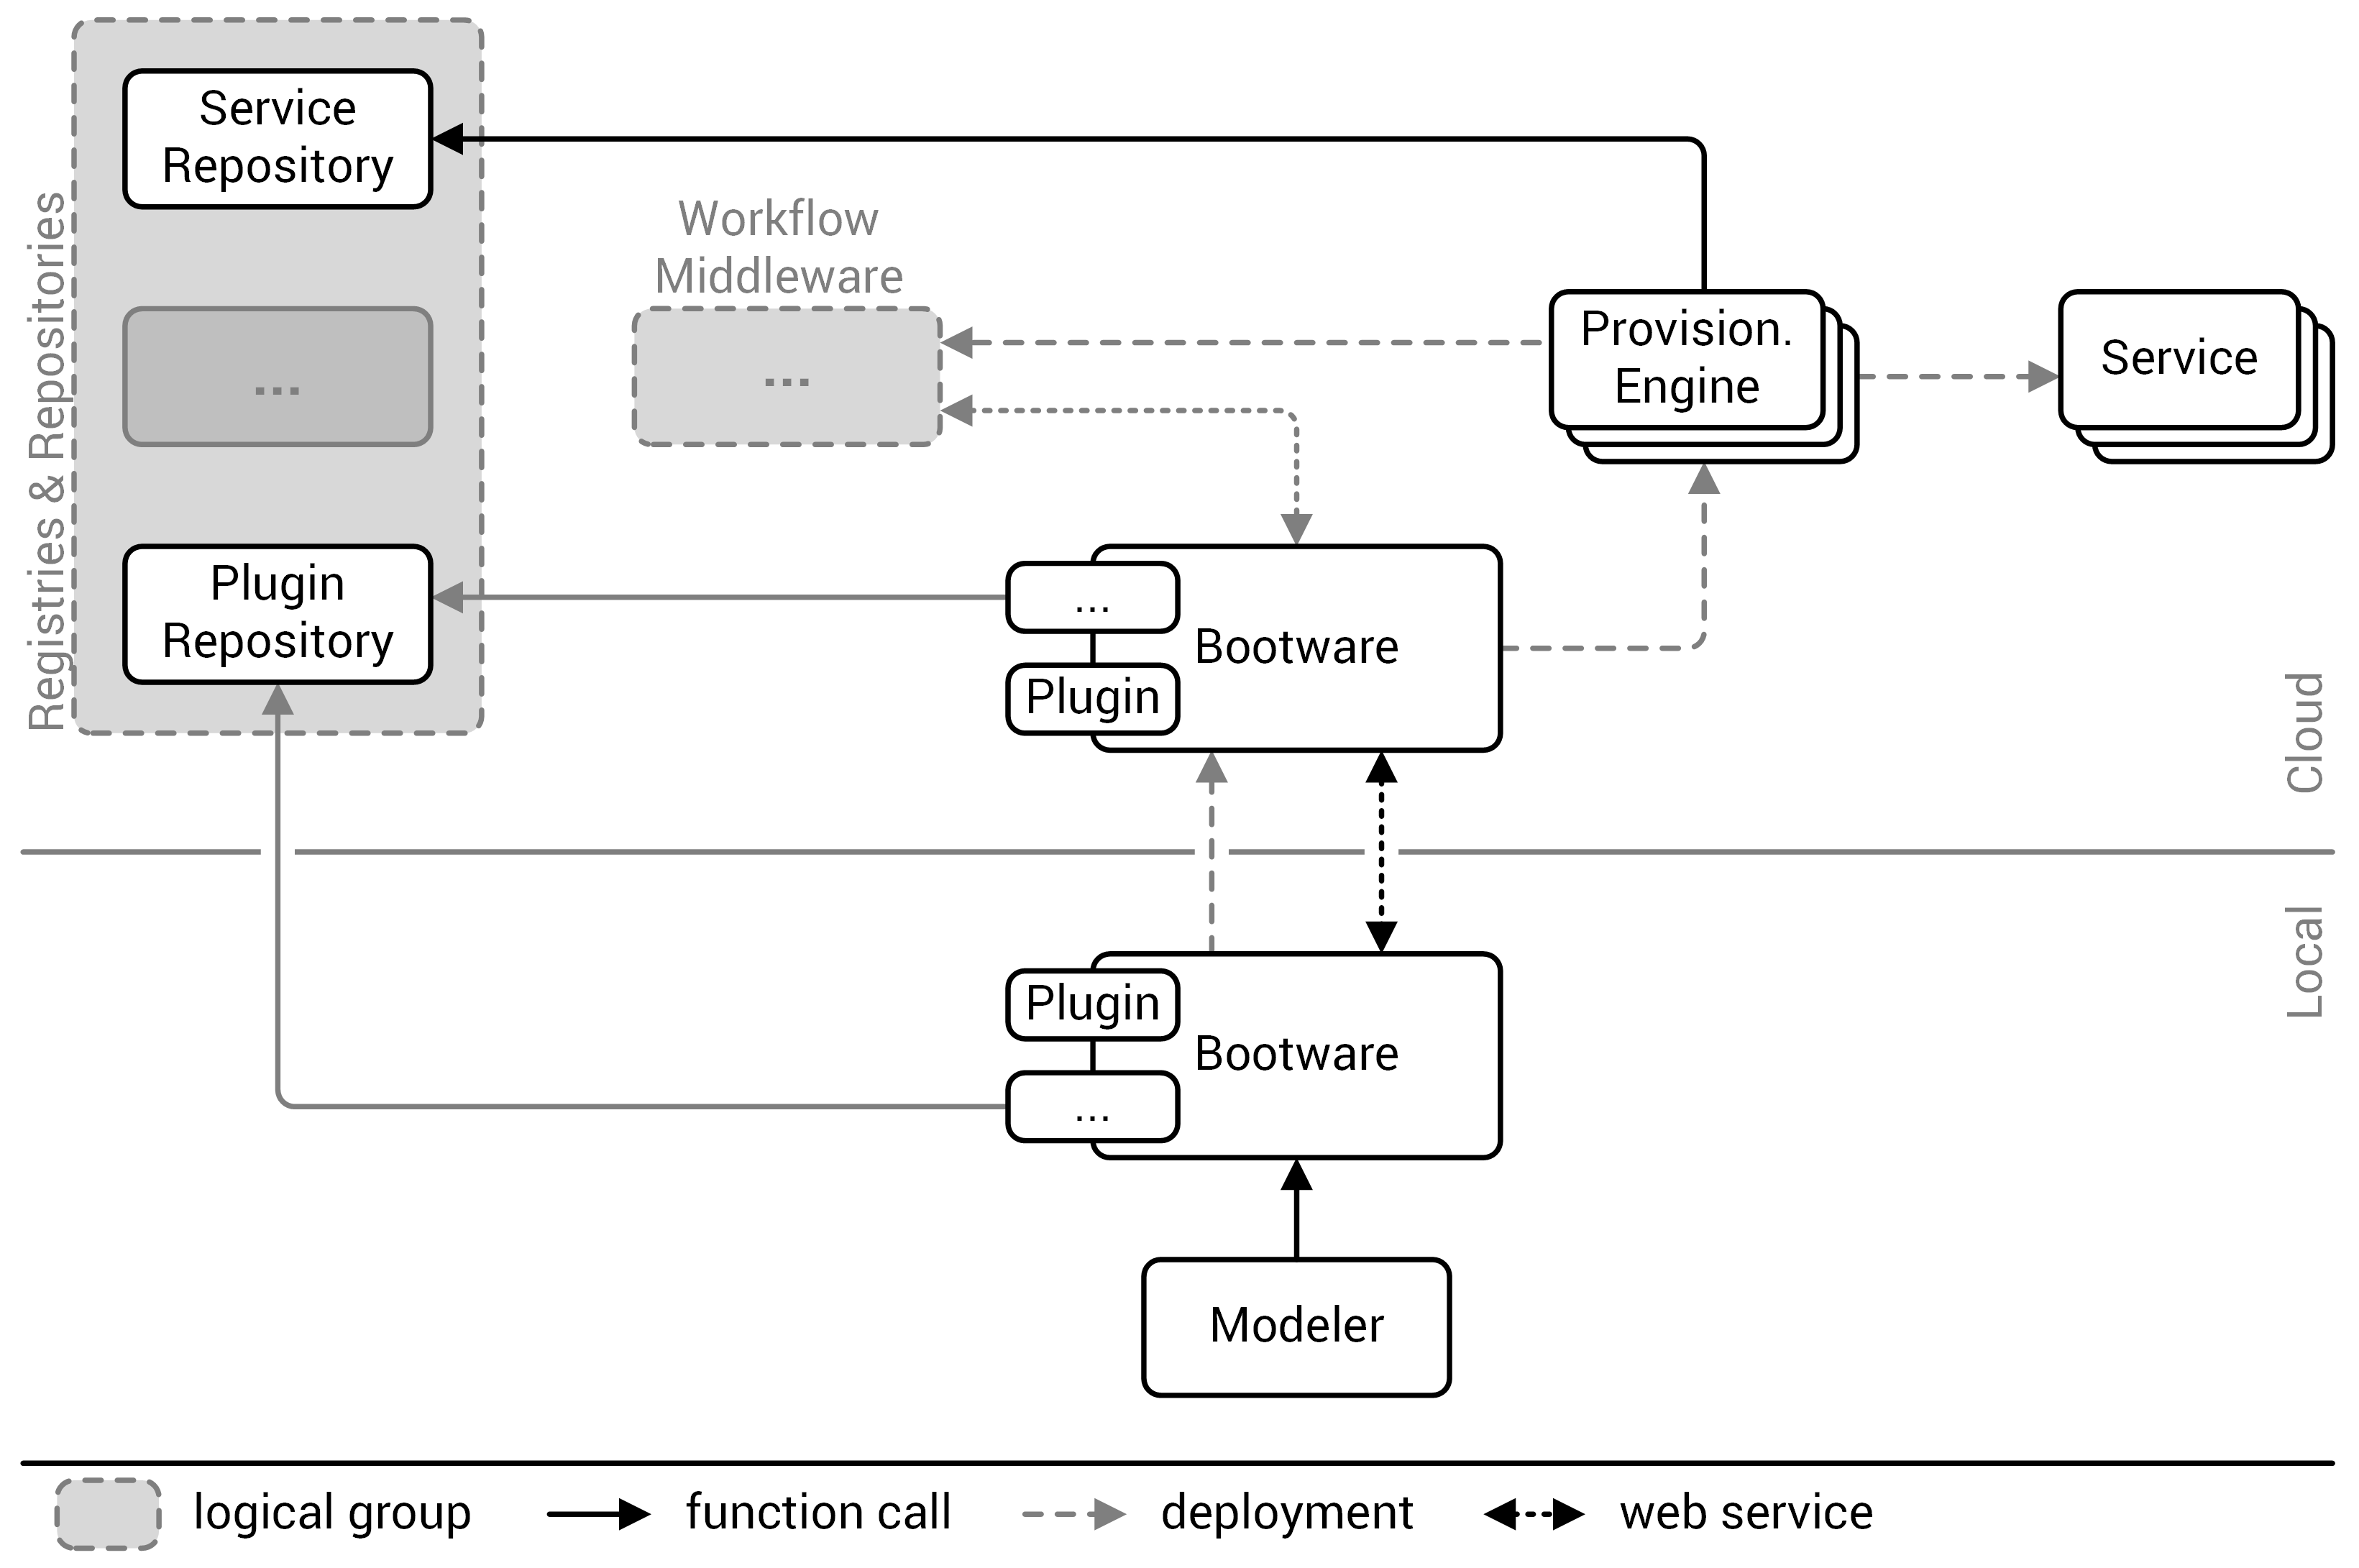
\includegraphics[resolution=600]{design/assets/simple_webservice}
	\caption{Simplified overview of the 2-tier architecture with asynchronous web service communication}
	\label{image:webservice}
\end{figure}

Since the provisioning processes kicked off by the bootware can potentially take a long time to finish (in the range of minutes to hours), asynchronous communication should be used between the components to avoid timeouts and blocking resources.
For the same reason, there should be some mechanism to get feedback on the current status during a long running provisioning process.

The communication with the bootware components will contain sensitive data, for example login information for cloud providers.
This information has to be provided from the outside on a call to call basis and should be transported securely to prevent malicious or fraudulent attacks.
The selected communication method therefore has to support some sort of security mechanism, ideally end-to-end encryption.
While these security mechanisms will not be used in this thesis due to time constraints, selecting the right communication method is still critical for future development.

Java provides a package for \nom{Remote Method Invocation}{RMI}, which allows object in one Java VM to invoke methods on objects in another Java VM~\autocite{rmi}.
But since RMI is limited to Java and we might want to communicate with the bootware from a component written in another programming language, RMI doesn't seem like a good fit.
For communication between programs written in different languages we could use the \nom{Common Object Request Broker Architecture}{CORBA}, a standard defined by the \nom{Object Management Group}{OMG}.
It supports mappings for common programming languages, like Java, C++, Python, and others.
Corba also supports asynchronous method invocation via callbacks~\autocite{corba:async} and transport layer encryption and other security features~\autocite{corba:security}.
Another alternative are web services via \nom{Simple Object Access Protocol}{SOAP} or \nom{Representational State Transfer}{REST}.
Like CORBA, web services also support asynchronous invocation, as well as security mechanisms~\autocite{ws:security}.

\begin{figure}[!htbp]
	\centering
	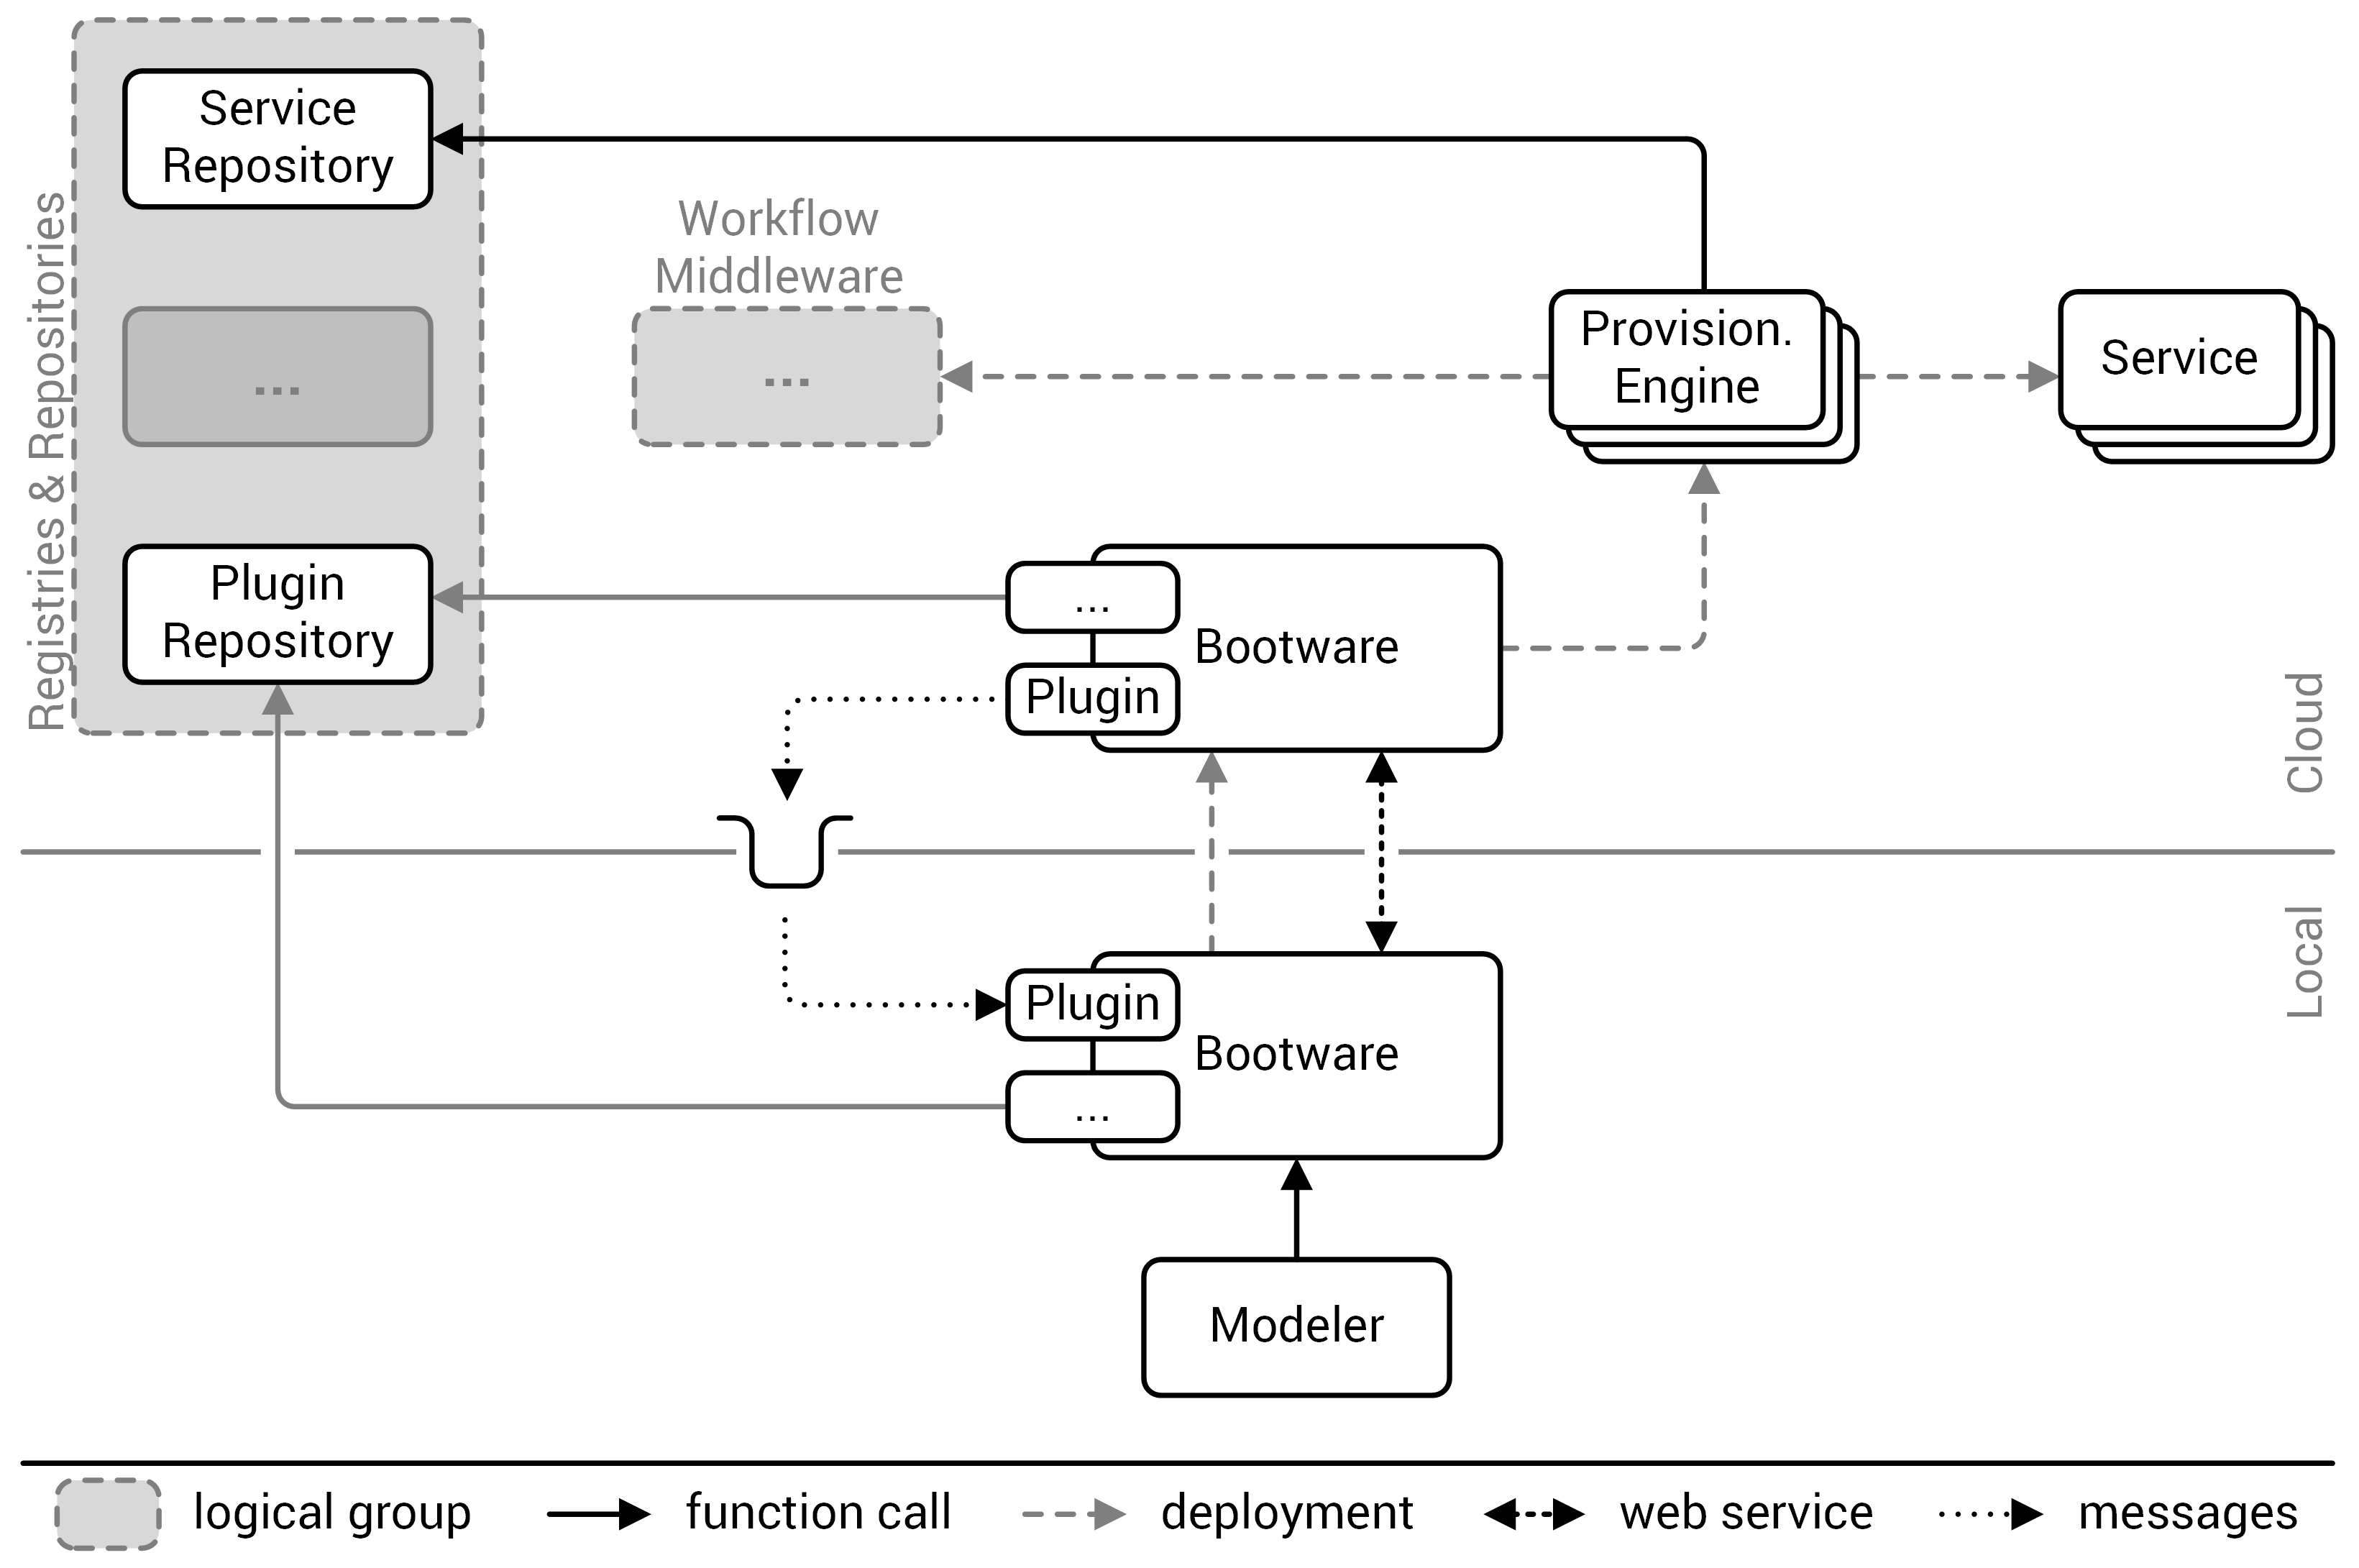
\includegraphics[resolution=600]{design/assets/simple_queue}
	\caption{Simplified overview of the 2-tier architecture with asynchronous web service and a messaging queue communication}
	\label{image:queue}
\end{figure}

Since the whole SimTech SWfMS already uses SOAP based web service, it would make sense to also use SOAP based web services as external communication mechanism for the bootware component.
The technology and knowledge is already in place and introducing a second mechanism like CORBA would unnecessarily increase the complexity of the project, especially since CORBA doesn't offer any significant advantages over SOAP based web services.
\autoref{image:webservice} shows the addition of asynchronous web service call and return communication to the proposed architecture.

With asynchronous communication, long running provisioning processes won't pose a problem.
We do however still need information during those long running processes to give the user some feedback.
This can't be accomplished by the simple web service request/response pattern.
For this, a secondary communication mechanism which supports sending multiple feedback messages has to be used.

Since it is not necessary for the successful use of the bootware it would make sense to implement this secondary communication mechanism as a plugin.
This would allow us to add arbitrary communication plugins to the bootware depending on future needs.
These secondary communication channels could take any form, but a natural choice for publishing the intermediary state of the bootware would be a message queue system.
In this case, the remote bootware component pushes messages to a message queue to which the local bootware component (and other components if needs be) can subscribe to receive future messages.
\autoref{image:queue} shows the proposed architecture with an additional message queue.

\subsection{Web Service Interface}

Now that we know that we'll use web service calls and returns as external communication mechanism, we need to the define the interface that will be made available by the web service to the outside.
We obviously need the two main operations, deploy and undeploy, to be available from the outside.

\subsubsection{Deploy}

The \textit{deploy} operation will be called by at least three different components.
Once by the bootware modeler plugin to deploy the remote bootware, \textcolor{red}{once again when the provisioning engine for provisioning the workflow middleware is deployed}, and then each time the provisioning manager needs to provision a new service during a workflow execution.

\vspace{1em}
\begin{listing}[!htbp]
	\inputminted[
		label=deploy-request.xml,
		frame=topline,
		linenos,
		frame=lines,
		tabsize=2,
		framesep=0.3cm,
		fontsize=\small
	]{xml}{design/assets/deploy-request.xml}
	\caption{Sample deploy request in a soap message.}
	\label{lst:webservice:deployrequest}
\end{listing}

\autoref{lst:webservice:deployrequest} shows an exemplary deploy request as soap message.
In line 6 we can see that the deploy method is called with the context provided as argument in line 7-11.
The response that is return once the request has been executed successfully is shown in \autoref{lst:webservice:deployresponse}.
It contains a endpoint reference element in line 6-9 which contains a reference to the payload that was deployed during the request.

\vspace{1em}
\begin{listing}[!htbp]
	\inputminted[
		label=deploy-response.xml,
		frame=topline,
		linenos,
		frame=lines,
		tabsize=2,
		framesep=0.3cm,
		fontsize=\small
	]{xml}{design/assets/deploy-response.xml}
	\caption{Sample deploy response in a soap message.}
	\label{lst:webservice:deployresponse}
\end{listing}

\subsubsection{Undeploy}

Like the \textit{deploy} operation, the \textit{undeploy} operation will be called by multiple components to reverse the actions that where previously made by deploy operations.
\autoref{lst:webservice:undeployrequest} shows an exemplary undeploy request in a soap message.
As argument it contains one or more endpoint references to already deployed payloads, as can be seen in line 7-13.
When all payloads have been undeployed successfully, a response will be send to.

\vspace{1em}
\begin{listing}[!htbp]
	\inputminted[
		label=undeploy-request.xml,
		frame=topline,
		linenos,
		frame=lines,
		tabsize=2,
		framesep=0.3cm,
		fontsize=\small
	]{xml}{design/assets/undeploy-request.xml}
	\caption{Sample undeploy request in a soap message.}
	\label{lst:webservice:undeployrequest}
\end{listing}

\subsubsection{SetCredentials}

In addition to the main deploy and undeploy operations, the bootware web service also supports the \textit{setCredentials} operation.
Using this operation, login credentials can be set independently from deploy requests if necessary.
\autoref{lst:webservice:setCredentialsrequest} shows an exemplary set credentials request.
In line 7-14, it contains one or more credentials as argument.
If the credentials where set successfully, a response will be returned.

\vspace{1em}
\begin{listing}[!htbp]
	\inputminted[
		label=setCredentials-request.xml,
		frame=topline,
		linenos,
		frame=lines,
		tabsize=2,
		framesep=0.3cm,
		fontsize=\small
	]{xml}{design/assets/setCredentials-request.xml}
	\caption{Sample setCredentials request in a soap message.}
	\label{lst:webservice:setCredentialsrequest}
\end{listing}
